% 中文摘要      I_chabstract.tex
% 英文摘要      II_enabstract.tex
% 誌謝          III_acknowledge.tex

% 主程式                00_masterthesis.tex
% 緒論                  01_introduction.tex
% 背景知識與相關文獻    02_relatedwork.tex
% 問題分析              03_analysis
% 研究方法              04_method.tex
% 實驗與結果分析        05_experiment.tex
% 結論                  06_conclusion.tex
% 附錄                  07_appendix.tex

% clean.bat 為清除、複製檔案於 C:\xtemp 使用。
% IEEEtran.sty 為文獻格式必須檔。
% *.bib 為文獻檔

%%%%%%%%%%%%%%%%%%%%%%%%%%%%%%%%%%%%%%%%%%%%%%%%%%%%%%%%%%%%%%%%%%%%%%%%%%%%%%%%%%%%%%%%%%%%%%%%%%%%
\documentclass[12pt,oneside,openany,a4paper,draft=FALSE]{book}

% 套件集
%\usepackage[left=3cm,top=3cm,nohead]{geometry}
%\usepackage[total={15cm,24cm}, top=35mm, left=36mm, includefoot]{geometry}
\usepackage[total={15cm,24cm}, top=30mm, left=30mm, includefoot]{geometry}  %版面格式

\usepackage{times}
\usepackage{titlesec}
\usepackage{caption}
\usepackage{comment}
\usepackage{bm}
%\usepackage[usenames,dvipsnames]{color}     %自訂文字顏色
\usepackage{graphicx,subfigure,float}       % 所有圖片均為浮動狀態,可為圖片編碼
\usepackage{amsmath,amssymb}                % 數學式
%\usepackage{color,colortbl,lettrine,wrapfig}
%\usepackage{epstopdf} %EPS轉PDF功能
%\usepackage[bookmarks=false,colorlinks=true,breaklinks=true]{hyperref} %PDF書籤與連結功能
\usepackage[numbered]{bookmark} %PDF書籤與連結功能
\usepackage[titletoc]{appendix}
%\usepackage{breakurl}

% 文獻套件
\usepackage[square,numbers]{natbib} %中英文文獻
%\usepackage{natbib}
\usepackage{bibentry}
%\usepackage{biblatex}
%\usepackage[notocbib]{apacite}     % use APA citation
%\usepackage{IEEEtran}   %IEEE文獻
\usepackage[notindex,nottoc,notlot,notlof]{tocbibind}

\usepackage{longtable}
\usepackage{url}
\usepackage{wallpaper}     % 浮水印

% 表格套件
\usepackage{array}
\usepackage{fancyhdr}
\usepackage{rotating}   % 旋轉表格,將某頁版面由直排轉為橫排,適合用於旋轉占滿一頁的表格或圖形
\usepackage{booktabs}
%\usepackage{graphicx,floatrow}

% 數學
\usepackage{amsthm}     % 排版數學文稿的定理與定義
\usepackage{amsmath}
\usepackage{enumerate}  % 條列項目 (阿拉伯數字編號)

%% 中文專用
\usepackage{fontspec} %加這個就可以設定字體
\usepackage{xeCJK} %讓中英文字體分開設置

%-----

% 設定『目錄』名稱
\renewcommand{\contentsname}{目錄}
\renewcommand{\listfigurename}{圖目錄}
\renewcommand{\listtablename}{表目錄}
%\renewcommand{\appendixtocname}{附錄}   % if \appendix  is used.
\renewcommand{\appendixname}{附錄}   % if \appendix  is used.
\renewcommand{\tablename}{表}
\renewcommand{\figurename}{圖}
\renewcommand{\bibname}{參考文獻}

\hypersetup{
    bookmarks=true,         % show bookmarks bar?
    colorlinks=true,        % false: boxed links; true: colored links
    linkcolor=red,          % color of internal links (change box color with linkbordercolor)
    citecolor=red,          % color of links to bibliography
    filecolor=cyan,         % color of file links
    urlcolor=magenta        % color of external links
}

%\newcommand{\img}{C:/Dropbox/ntpu_thesis/plot/}%如果所有圖檔存放在其他地方,先定義位置

\pagestyle{fancy}
\fancyhf{}
\renewcommand{\chaptermark}[1]{\markboth{\thechapter .\ #1}{}}  % 去除章編號前後的字
\titleformat{\chapter}[display]{\center\LARGE\sf}{第\ \thechapter\ 章}{0.2cm}{}  %設計章節標題式樣,標題置中
\titlespacing{\chapter}{0pt}{-50pt}{25pt}   %設計章節標題式樣,控制間距
%\fancyhead[RO,RE]{\leftmark}   %章節標題於頁眉/頁足上
\fancyfoot[CO,CE]{\thepage}

\renewcommand{\headrulewidth}{0pt}  % 頁眉下方的橫線
%\renewcommand{\footrulewidth}{0pt} % 設定頁首多一條粗細是 0.4 pt 的水平線

% 設定itemize符號
\renewcommand{\labelitemi}{$\bullet$}
\renewcommand{\labelitemii}{$\circ$}

%設定英文字型,不設的話就會使用預設的字型
\setmainfont{Times New Roman}

% 設定中文字體
\setCJKmainfont{標楷體} %設定中文為系統上的字型,而英文不去更動,使用原TeX字型
%\setCJKmainfont{cwTeXKai}
\XeTeXlinebreaklocale "zh"
\XeTeXlinebreakskip = 0pt plus 1pt %這兩行一定要加,中文才能自動換行


\renewcommand{\baselinestretch}{1.25}   %依照文章預設行距增加為 1.25倍(不同字型大小行距值,加大為1.25倍)

% 以下是目錄章節後面打點格式的設定:http://vardesa.blog.hexun.com.tw/58537832_d.html
\makeatletter
\def\@bfdottedtocline#1#2#3#4#5{%
\ifnum #1>\c@tocdepth \else
\vskip \z@ \@plus.2\p@
{\leftskip #2\relax \rightskip \@tocrmarg \parfillskip -\rightskip
\parindent #2\relax\@afterindenttrue
\interlinepenalty\@M
\leavevmode \bfseries
\@tempdima #3\relax
\advance\leftskip \@tempdima \null\nobreak\hskip -\leftskip
{#4}\normalfont\nobreak
\leaders\hbox{$\m@th
\mkern \@dotsep mu\hbox{.}\mkern \@dotsep
mu$}\hfill
\nobreak
\hb@xt@\@pnumwidth{\hfil\normalfont \normalcolor #5}%
\par}%
\fi}
\renewcommand*\l@chapter{\@bfdottedtocline{0}{0em}{1.5em}}
\makeatother

% 定義『各章節標題、圖表、頁尾註記』字型

\theoremstyle{plain}   % 排版格式,{plain}:最醒目格式
\newtheorem{thm}{定理}  % 將 Theorem 改為國字「定理」
\newtheorem{thmm}{定義}


%
%   調整內縮長度(依據學校規定與不同版面、字型調整)
%
\parindent=0.85cm
%% 修改中文標題與格式定義
\date{2013.9.18}    %版本日期

%%%%% 論文開始 %%%%%
\begin{document}

%%  封面
%% 封面頁
\fontsize{24}{20pt}\selectfont
\thispagestyle{empty}

\begin{center}
        
\includegraphics[width=3.43cm,height=3.43cm]{graphs/logo/logo.eps}\\
	\huge 國立高雄大學電機工程學系 \\  大專生畢業專題論文
\end{center}

\vspace*{1cm}

\begin{center}
	\fontsize{24}{18pt}
	\LARGE 人工智慧結合機械手臂於智慧撞球之應用 \\

	Application of Artificial Intelligence Combined with Robotic Arm in Billiard Game
\end{center}

\vspace*{0.5cm}

\begin{center}
	\fontsize{24}{18pt}
	\LARGE 專題生:邱繼群、林子晧\  撰\\
	\LARGE 指導教授:吳志宏\ 博士 \\
\end{center}

\vspace*{0.5cm}

\begin{center}
	\LARGE 中華民國\ 一百一十\ 年\ 十二\ 月
\end{center}

\newpage



\CenterWallPaper{0.17}{graphs/logo/logowatermark.eps} %浮水印
%===============================================================
%%%%%%%%%%%%%%%%---------- 中文摘要
\frontmatter % 羅馬文頁碼
\newpage
%\thispagestyle{empty} %不出現頁碼
\phantomsection
\addcontentsline{toc}{chapter}{中文摘要} %手動加入目錄文字
    \fontsize{12}{18pt}\selectfont

    \begin{center}
        \LARGE 人工智慧結合機械手臂於智慧撞球之應用 \\
    \end{center}

    \vspace*{0.25cm}

    {\small
        \begin{center}
        指導教授: 吳志宏\ 博士 \\
        學生: 邱繼群、林子晧\  \\
        國立高雄大學電機工程學系
        \end{center}
    }

    \vspace*{0.25cm}

    \begin{center}
        {\large \bf 摘要}\\[12pt]
    \end{center}
    \hspace{7mm}
	工業4.0的來臨,對於人工智慧及機械手臂的技術需求越來越多,為能夠在資源及
	時間有限的情況能夠確實研究機械手臂結合人工智慧之技術,並且以有趣且簡單的
	方式呈現於專題之中,我們選擇上銀機械手臂比賽中智慧撞球項目作為專題研究主
	題,希望透過影像辨識、機械手臂與氣缸控制的結合,藉次模擬人類打撞球的思維
	及行爲。
    \vspace{5mm}

    \noindent
    關鍵字:影像辨識、人工智慧、機械手臂、YOLO。




%%%%%%%%%%%%%%%%---------- 英文摘要
\newpage
%\thispagestyle{empty} 不出現頁碼
\phantomsection
\addcontentsline{toc}{chapter}{英文摘要} %手動加入目錄文字
    \fontsize{12}{13pt}\selectfont

    \begin{center}
        \LARGE
	Application of Artificial Intelligence Combined with Robotic Arm in Billiard Game

    \end{center}

    \begin{center}
        \small Advisor: Dr. WU, CHI-HUNG \\
        Student: CHIU, CHI-CHUN \ \
				LIN,ZI-HAO\\
        Department of Electrical Engineering, National University of Kaohsiung
    \end{center}

    \begin{center}
        {\large \bf ABSTRACT}
    \end{center}
    \hspace{7mm}
    \fontsize{8}{15pt}
	With the advent of Industry 4.0,
    \vspace{5mm}

    \noindent Keywords: Image Recognition, Artificial Intelligence, Robotic Arm, YOLO.


%%%%%%%%%%%%%%%%---------- 致謝
\newpage
%\thispagestyle{empty} 不出現頁碼
\addcontentsline{toc}{chapter}{致謝} %手動加入目錄文字
    \begin{center}
        \huge{致謝}
    \end{center}

    \fontsize{12}{18pt}\selectfont
    \hspace{7mm}
        致謝,致謝,致謝,致謝,
        致謝,致謝,致謝,致謝,
        致謝,致謝,致謝,致謝,
        致謝,致謝,致謝,致謝,
        致謝,致謝,致謝。
    \vspace*{15mm}

    \begin{flushright}
       ○○○ 謹誌於○○○○大學○○○○系 \\   中華民國一零○年○月
    \end{flushright}


%%  目錄
\newpage
%%\newpage
\fontsize{12}{18pt}\selectfont
%%  目錄
\phantomsection
\addcontentsline{toc}{chapter}{目錄} %手動加入目錄文字
\tableofcontents
\newpage
%%  圖目錄
%%\phantomsection
%%\addcontentsline{toc}{chapter}{圖目錄} %手動加入目錄文字
%%\listoffigures
%%\newpage
%%%%  表目錄
%%\phantomsection
%%\addcontentsline{toc}{chapter}{表目錄} %手動加入目錄文字
%%\listoftables
%%\newpage


%%%%%%%%%%%%%%%%%%%% 碩士論文內文開始 %%%%%%%%%%%%%%%%%%%%

%%%%%%%%%%%%%%%%---------- 開始章節
\cleardoublepage
\mainmatter % 阿拉伯文頁碼
\fontsize{12}{21pt}\selectfont

%%  緒論
\chapter{緒論}
\label{chapter:intro}
\section{研究背景與動機}
\label{sec:background}
    \subsection{子章節一}
        字章節一段落一,字章節一段落一,字章節一段落一,字章節一段落一,
        字章節一段落一,字章節一段落一,字章節一段落一,字章節一段落一,
        字章節一段落一,字章節一段落一,字章節一段落一,字章節一段落一,
        字章節一段落一,字章節一段落一,字章節一段落一,字章節一段落一,
        字章節一段落一,字章節一段落一,字章節一段落一。

        字章節一段落二,字章節一段落二,字章節一段落二,字章節一段落二,
        字章節一段落二,字章節一段落二,字章節一段落二,字章節一段落二,
        字章節一段落二,字章節一段落二,字章節一段落二,字章節一段落二,
        字章節一段落二,字章節一段落二,字章節一段落二,字章節一段落二,
        字章節一段落二,字章節一段落二,字章節一段落二,字章節一段落二,
        字章節一段落二,字章節一段落二,字章節一段落二,字章節一段落二,
        字章節一段落二。

        例如現有的系統有\cite{GoogleComputeEngine}、\cite{AmazonEC2}等等,
        另外\cite{GoogleApps}是以○○○技術來達成。

        ○○系統結構如示意圖\ref{fig:this_system}
        \begin{figure}[htbp]
            \centerline{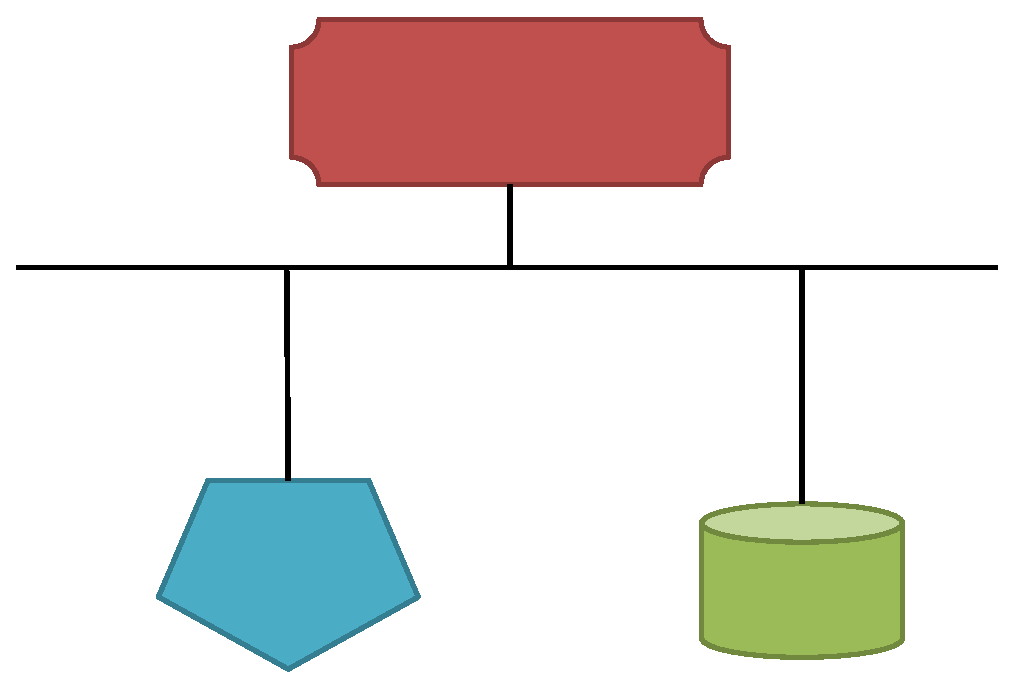
\includegraphics[height=5cm]{graphs/introduction/this_system.eps}}
            \caption{○○示意圖}
            \label{fig:this_system}
        \end{figure}

    \subsection{子章節二}
        字章節二,字章節二,字章節二,字章節二,字章節二,
        字章節二,字章節二,字章節二,字章節二,字章節二,
        字章節二,字章節二,字章節二,字章節二,字章節二,
        字章節二,字章節二,字章節二,字章節二,字章節二,
        字章節二,字章節二,字章節二,字章節二,字章節二,
        字章節二,字章節二,字章節二,字章節二,
        ○○○如圖~\ref{fig:types_comparison}所示。
        \begin{figure}[!t]
            \begin{center}
                \begin{tabular}{ccccccccccccc}
                    \subfigure[類型A]{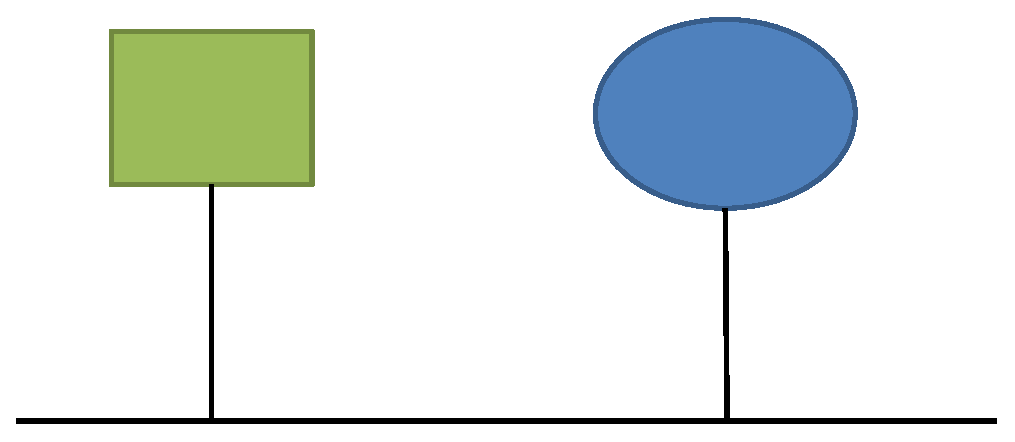
\includegraphics[height=2.4cm]{graphs/introduction/typeA.eps}\label{fig:typeA} } \par &
                    \subfigure[類型B]{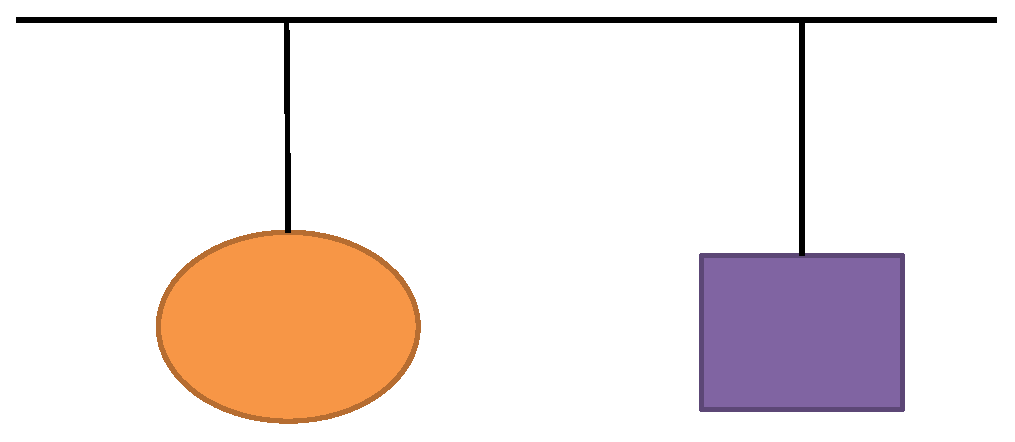
\includegraphics[height=2.4cm]{graphs/introduction/typeB.eps}\label{fig:typeA} } \par \\
                \end{tabular}
                \caption{○○○比較}
                \label{fig:types_comparison}
            \end{center}
        \end{figure}

\section{○○○問題與處理機制}
    問題與機制,問題與機制,問題與機制,問題與機制,
    問題與機制,問題與機制,問題與機制,問題與機制,
    問題與機制,問題與機制,問題與機制,問題與機制,
    問題與機制,問題與機制,問題與機制,問題與機制,
    問題與機制。

    %要被單行註解的文字。

\begin{comment}
    要被區塊註解的文字,要被區塊註解的文字,要被區塊註解的文字,
    要被區塊註解的文字,要被區塊註解的文字,要被區塊註解的文字,
    要被區塊註解的文字,要被區塊註解的文字,要被區塊註解的文字,
    要被區塊註解的文字,要被區塊註解的文字,要被區塊註解的文字,
    要被區塊註解的文字,要被區塊註解的文字,要被區塊註解的文字,
    要被區塊註解的文字,要被區塊註解的文字。
\end{comment}

\section{研究動機與目的}
    動機與目的,動機與目的,動機與目的,動機與目的,
    動機與目的,動機與目的,動機與目的,動機與目的,
    動機與目的,動機與目的,動機與目的,動機與目的,
    動機與目的,動機與目的,動機與目的,動機與目的,
    動機與目的,動機與目的,動機與目的,
    細節如表\ref{tab:mytitle1}。
    \begin{table}[!t]
        \centering
        \caption{表格標題1}
        \label{tab:mytitle1}
        % Table generated by Excel2LaTeX from sheet 'table_01'
\begin{tabular}{rr}
\toprule
Title & Values \\
\midrule
A     & 1612 \\
B     & 256 \\
C     & 30 \\
D     & 7 \\
E     & 3 \\
\bottomrule
\end{tabular}%

    \end{table}

    \begin{enumerate}
        \item
        列舉一。
        %
        \item
        列舉二。
        %
        \item
        列舉三。
        %
    \end{enumerate}

\section {研究方法與論文架構}
    研究方法與論文架構,研究方法與論文架構,研究方法與論文架構,
    研究方法與論文架構,研究方法與論文架構,研究方法與論文架構,
    研究方法與論文架構,研究方法與論文架構,研究方法與論文架構,
    研究方法與論文架構。

    \begin{itemize}
        \item
        項目一。
        %
        \item
        項目二。
        %
        \item
        項目三。
        %
        \item
        項目四。
    \end{itemize}

    流程圖如\ref{fig:ResearchFlowChart}。
    \begin{figure}[htbp]
        \centering
        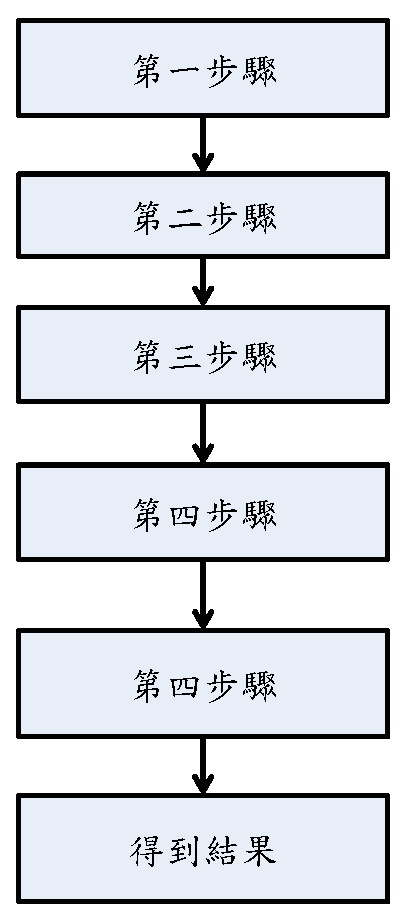
\includegraphics[height=8cm]{graphs/introduction/ResearchFlowChart.eps}
        \caption{研究進行流程圖}
        \label{fig:ResearchFlowChart}
    \end{figure}



%%  背景知識與相關文獻
\chapter{文獻探討}
\label{chapter:literature}
本章簡述研究應用之相關技術與相關文獻探討。

\section{○○○系統之文獻探討}
    ○○○系統,○○○系統,○○○系統,○○○系統,
    ○○○系統,○○○系統,○○○系統,○○○系統,
    ○○○系統,○○○系統,○○○系統,○○○系統,
    ○○○系統,○○○系統,○○○系統。

    如文獻\cite{chen:2011}與\cite{hsiao:2013}所提出之○○○;
    而\cite{wan:2010}則認為○○○。

    在國外則有\cite{collobert:2001}、\cite{mell:2011}所提出之○○○相關研究。

\section{○○○技術之文獻探討}
    ○○○技術,○○○技術,○○○技術,○○○技術,○○○技術,
    ○○○技術,○○○技術,○○○技術,○○○技術,○○○技術,
    ○○○技術,○○○技術,○○○技術,○○○技術,○○○技術,
    ○○○技術,○○○技術,○○○技術,○○○技術,○○○技術,
    ○○○技術,○○○技術。


%%  問題定義與分析
\chapter{問題定義與分析}
\label{chapter:analysis}
    本研究所探討的○○○○○:
    第一階段將討論○○○○,
    第二階段則說明○○○○。

\section{○○○定義}
    ○○○定義,○○○定義,○○○定義,
    ○○○定義,○○○定義,○○○定義,
    ○○○定義,○○○定義,○○○定義,
    ○○○定義,○○○定義,○○○定義,
    ○○○定義,○○○定義,○○○定義,
    ○○○定義,○○○定義。
    
    ○○○定義,○○○定義,○○○定義,
    ○○○定義,○○○定義,○○○定義,
    ○○○定義,○○○定義,○○○定義,
    ○○○定義,○○○定義。

\section{○○○分析}
    ○○○分析,○○○分析,○○○分析,○○○分析,
    ○○○分析,○○○分析,○○○分析,○○○分析,
    ○○○分析,○○○分析,○○○分析,○○○分析,
    ○○○分析,○○○分析,○○○分析,○○○分析,
    ○○○分析,○○○分析,○○○分析,○○○分析,
    ○○○分析,○○○分析,○○○分析,○○○分析,
    ○○○分析,○○○分析,○○○分析。



%%  研究設計與方法
\chapter{研究方法與設計}
\label{chapter:method}

\section{研究方法}
    研究方法,研究方法,研究方法,研究方法,
    研究方法,研究方法,研究方法,研究方法,
    研究方法,研究方法,研究方法,研究方法,
    研究方法,研究方法,研究方法,研究方法,
    研究方法。

\section{處理機制}
    處理機制,處理機制,處理機制,處理機制,處理機制,
    處理機制,處理機制,處理機制,處理機制,處理機制,
    處理機制,處理機制,處理機制,處理機制,處理機制,
    處理機制,處理機制,處理機制,處理機制,處理機制,
    處理機制,處理機制,處理機制。



%%  實驗與結果分析
\chapter {實驗與結果分析}
\label{chapter:experiments}

\section{實驗環境與架構}
    實驗環境與架構,實驗環境與架構,實驗環境與架構,實驗環境與架構,
    實驗環境與架構,實驗環境與架構,實驗環境與架構,實驗環境與架構,
    實驗環境與架構,實驗環境與架構,實驗環境與架構,實驗環境與架構,
    實驗環境與架構,實驗環境與架構,實驗環境與架構,實驗環境與架構,
    實驗環境與架構,實驗環境與架構,實驗環境與架構,實驗環境與架構,
    實驗環境與架構。

\section{○○○分析之比較}
    ○○○分析之比較,○○○分析之比較,○○○分析之比較,
    ○○○分析之比較,○○○分析之比較,○○○分析之比較,
    ○○○分析之比較,○○○分析之比較,○○○分析之比較,
    ○○○分析之比較,○○○分析之比較,○○○分析之比較,
    ○○○分析之比較,○○○分析之比較,○○○分析之比較。

\section{○○○策略之比較}
    ○○○策略之比較,○○○策略之比較,○○○策略之比較,○○○策略之比較,
    ○○○策略之比較,○○○策略之比較,○○○策略之比較,○○○策略之比較,
    ○○○策略之比較,○○○策略之比較,○○○策略之比較,○○○策略之比較,
    ○○○策略之比較,○○○策略之比較,○○○策略之比較,○○○策略之比較,
    ○○○策略之比較,○○○策略之比較。











































\begin{comment}
\chapter {實驗與結果分析}
    本研究目的為使用圖形處理器加速演化式硬體影像濾波器的計算,
    並嘗試各種對演化式硬體的結果有影響的組合,
    最後進行實驗數據的比較與分析。
    第一小節為實驗環境與架構,
    說明實驗環境與實驗對象。
    其後各小節為實驗結果,
    並於最後一小節做實驗結論。

\section{實驗環境與架構}
\hspace{7mm}
    實驗環境為一台4核心 (執行緒數量為 8)電腦,
    CPU型號為 Intel Core i7-3770, 3.4GHz,
    記憶體大小為 8GB,
    程式開發軟體為 C語言。
    在 GPU部分,
    GPU型號為 Tesla C1060, 800 MHz,
    GPU記憶體為 4GB,
    處理器核心數量共 240顆,
    程式開發軟體為 CUDA,
    硬體計算能力版本為 1.3。
    匯流排為 PCI-E2.0,
    傳輸速度為 16GB/s。
    處理雜訊對象為胡椒鹽雜訊 (salt-and-pepper noise, SPNoise)及
    脈衝雜訊 (impulse bursts noise, IBNoise)。
    胡椒鹽雜訊為在影像上隨機分佈白點與黑點像素,
    而脈衝雜訊為連續的白色像素。
    請參考圖\ref{fig:0501NoiseSample}。
    實驗測試影像則選定三張標準測試影像,
    如圖\ref{fig:0501TestingImage},
    影像資料為 8-bits灰階圖。

    \begin{figure}[tbp]
        \centering
        \subfigure[原始影像]{\includegraphics[width=2.7cm,bb=0 0 256 256]{graph/exp/01_Lena.png}}\hfill
        \subfigure[胡椒鹽雜訊]{\includegraphics[width=2.7cm,bb=0 0 256 256]{graph/exp/01_SPSample.png}} \hfill
        \subfigure[脈衝雜訊]{\includegraphics[width=2.7cm,bb=0 0 256 256]{graph/exp/01_IBSample.png}} \hfill
        %%
        \caption{雜訊影像}
        \label{fig:0501NoiseSample}
    \end{figure}

    \begin{figure}[tbp]
        \centering
        \subfigure[Cameraman]{\includegraphics[width=2.7cm,bb=0 0 256 256]{graph/exp/01_Cameraman.png}} \hfill
        \subfigure[Goldhill]{\includegraphics[width=2.7cm,bb=0 0 256 256]{graph/exp/01_Goldhill.png}}\hfill
        \subfigure[Lena]{\includegraphics[width=2.7cm,bb=0 0 256 256]{graph/exp/01_Lena.png}}\hfill
        %%
        \caption{測試影像}
        \label{fig:0501TestingImage}
    \end{figure}

    在訓練階段使用原始影像與一張含有雜訊的影像,
    CGP的函式如表\ref{tab:0202CGPFunctionTable}所列,
    將含有雜訊的影像還原後,
    再與原始影像比較,
    以 PSNR值為評估標準如公式(\ref{eq:PSNR_1}),
    藉以得知影像濾波器的好壞程度,
    並在演化結束後將擁有最高的 PSNR值當作此次實驗的最佳解。
    由於 PSNR值會受到演化式計算參數的不同而有高低,
    因此我們需要嘗試多種組合。

    在 GPU加速演化式硬體濾波器方面,
    我們考慮了 GPU在硬體與軟體上的限制如表\ref{tab:0402GPUTeslaParameters},
    在此限制上發揮 GPU計算的最大效能。

\section{實驗 A - 演化式硬體濾波器執行時間與分析}
\hspace{7mm}
    當 Population設為 100、Generation為 5000,
    交配與突變率分別為 60\%和 10\%,
    在遮罩大小為 $3 \times 3$與 $5 \times 5$下,
    演化式硬體濾波器的執行時間分別為 83693秒和 84967秒。

    執行一次演化式硬體濾波器需花費將近 24小時,
    在嘗試其他演化參數如交配與突變率或者增加 Generation都將窒礙難行,
    因此本實驗目的為找出時間花費最多的地方,
    執行方式為將演化式硬體濾波器的執行步驟拆解為:
    \begin{itemize}
        \item
        訓練階段-計算 Fitness:
        此步驟累計每代計算全部個體的時間。
        %
        \item
        訓練階段-產生個體:
        此步驟累計每代產生族群的時間,
        包含交配、突變以及重置。
        %
        \item
        訓練階段-其他步驟:
        和演化無關但卻需要執行的程式所花的時間。
        %
        \item
        測試階段:
        完成影像測試的時間花費。
    \end{itemize}

    各步驟所花時間如圖\ref{fig:0502CPUTimte}所示,
    由實驗數據得知計算 Fitness佔據最多時間,
    因此以 GPU加速此部分,
    加速方法請參考本論文第四章。

    \begin{figure}[tbp]
        \centering
        \includegraphics[width=0.9\columnwidth]{graph/exp/02_CPUTime.eps}
        \caption{一般執行下演化式硬體濾波器各步驟執行時間}
        \label{fig:0502CPUTimte}
    \end{figure}

\section{實驗 B - GPU參數對執行效率的結果與分析}
\hspace{7mm}
    本實驗以本論文第四章的方法設計演化式硬體濾波器,
    並分析 GPU的參數對本論文提出的設計架構的效率影響。
    演化式硬體濾波器的參數設計為表\ref{tab:0503CGP},
    取消重置機制讓每代計算的染色體數量相同,
    並以兩種遮罩大小$3 \times 3$和$5 \times 5$,
    當作執行效率的分析對象。

    \begin{table}[tbp]
      \centering
      \caption{實驗 B - CGP參數表}
      %
        \subtable[CGP共同參數]{
            \begin{tabular}{ll}
            \toprule
            Parameters & Value \\
            \midrule
            Image size & 256 $\times$ 256 \\
            CGP grid size & 8 $\times$ 4 \\
            Level back & 2 \\
            Number of function & 16 \\
            Stopping criteria & 5000 generations \\
            Population size & 100 \\
            \bottomrule
            \end{tabular}%
        }
        %
        \subtable[交配與突變機率]{
            \begin{tabular}{lcc}
            \toprule
                  & Crossover & Mutation \\
            \midrule
            CGP1  & 40\% & 40\% \\
            CGP2  & 60\% & 60\% \\
            CPG3  & 80\% & 80\% \\
            \bottomrule
            \end{tabular}%
        }
        %
      \label{tab:0503CGP}%
    \end{table}%

    當遮罩大小為 $3 \times 3$,
    代表遮罩數量為 $(256-3+1)^2$共 64516個。
    將一個遮罩的過濾交給一個 thread計算,
    共動用 64516個 thread。

    為了提高運算效率,
    以硬體的執行角度分析,
    分析過程的數據參考表\ref{tab:0503Analyzation1}。
    \begin{enumerate}
        \item
        一個 STMP內的共享記憶體空間為16384 bytes:
        影像為 8-bits灰階圖,
        所需要的共享記憶體空間為 $3^2 + 8 \times 4$共 41 bytes。
        代表一個 STMP內可用的 thread將被限制最多為 399個。
        %
        \item
        分組:
        thread需要 64516個但被限制為最多 399個,
        因此須分組成數個 block。
        若以質因數分解,
        64516可分解為:254、127、4、2、1,
        相對應的 block數量將為 254、508、\\
        16129、32258、64516。
        %
        \item
        Warp:
        STMP以 warp為單位執行,
        一個 warp由 32個 thread組成。
        若宣告的數量不足 32也會成為一個warp,
        代表有數個 thread的浪費。
        因此 254、127、4、2、1換成 warp的數量為8、4、1、1、1,
        thread的浪費量分別為 2、1、28、30、31。
        %
        \item
        Occupancy:
        為了減少延遲,
        需讓 STMP有足夠的 warp做文本切換。
        但有以下考量:
        \begin{itemize}
            \item
            一個 STMP最多只能放入 32個 warp:
            因此能使用的 block數量為 4、8、32、\\
            32、32。
            %
            \item
            一個 STMP內共享記憶體空間:
            因此能使用的 block數量為 1、2、99、199、399。
            (*共享記憶體會保留空間放執行的程式碼,
            因此無法全部使用。)
            %
            \item
            一個 STMP最多只能放入8個 block。
        \end{itemize}
        在上三點的限制下得到的 block數量為1、2、8、8、8。
        %
        \item
        綜合考量:
        考量 thread因包裝成 warp而造成的浪費與佔有率後,
        選擇 thread浪費最少的或者佔有率高的。
    \end{enumerate}

    \begin{table}[tbp]
      \centering
      \caption{GPU參數分析(遮罩大小為 $3 \times 3$)}
        \begin{tabular}{l|ccccc}
        \toprule
        Thread數量 & 254   & 127   & 4     & 2     & 1 \\
        \midrule
        warp & 8     & 4     & 1     & 1     & 1 \\
        Thread浪費量 & 2     & 1     & 28    & 30    & 31 \\
        \midrule
         & \multicolumn{5}{c}{換算成 block} \\
         \midrule
        STMP內最多共 32個 warp & 4     & 8     & 32     & 32     & 32 \\
        受限於共享記憶體的block數量 & 1     & 2*    & 99     & 199     & 399 \\
        \midrule
        warp $\times$ block & 8 $\times$ 1 & 4 $\times$ 2 & 1 $\times$ 8 & 2 $\times$ 8 & 3 $\times$ 8 \\
        佔有率   & 25\%  & 25\%  & 25\%  & 50\%  & 75\% \\
        \bottomrule
        \end{tabular}%
      \label{tab:0503Analyzation1}%
    \end{table}%

    實驗結果如圖\ref{fig:0503GPUTimeMask3},
    左邊縱軸為各種 thread設定下所花費的時間,
    以長條圖表示,
    單位為秒。
    右邊縱軸為各種 thread設定下的 speedup,
    speedup為 CPU與 GPU版本程式的時間比值,
    CPU版本程式所花費的時間呈現於圖上方的表格,
    以折線圖表示。
    從 thread數量來分析,
    可以發現在 thread數量為 254與 127的運算時間相差不多,
    但 thread數量為 127的時間較短,
    表示在相同的占有率下,
    浪費的 thread越少,
    運算效能越好。
    而在 thread數量為 4、2和1時,
    運算時間也為倍數差。
    從交配率來分析,
    比較交配率 40\%與 60\%的計算時間,
    兩者的時間倍數幾乎為 1.5倍,
    而 40\%與 80\%的計算時間幾乎為 2倍,
    表示本研究提出的方法很適合平行化計算。

    \begin{figure}[tbp]
        \centering
        \includegraphics[width=0.95\columnwidth]{graph/exp/03_GPUTimeMask3.eps}
        \caption{計算時間(秒) (遮罩大小為 $3 \times 3$)}
        \label{fig:0503GPUTimeMask3}
    \end{figure}

    而遮罩大小為 $5 \times 5$時,
    遮罩數量變成 $(256-5+1)^2$共63504,
    所需要的共享記憶體空間為 $5^2 + 8 \times 4$共 57 bytes。
    遮罩數量比 $3 \times 3$少,
    但一個thread所需的記憶體空間便多了,
    因此一個 STMP能容納的最大 thread將變少為 287個。
    而 63504可以拆解的質因數共有 38種,
    因此 thread有較多的選擇。
    但許多組合下 thread的浪費數量較多,
    在運算效能上的表現較差,
    因此只列出幾組數據討論。
    分析的方法同上敘述,
    分析結果請參考表\ref{tab:0503Analyzation2},
    實驗結果請參考圖\ref{fig:0503GPUTimeMask5}。

    \begin{table}[tbp]
      \centering
      \caption{GPU參數分析(遮罩大小為 $5 \times 5$)}
        \begin{tabular}{l|ccccc}
        \toprule
        Thread數量          & 252   & 189    & 144   & 63    & 48 \\
        \midrule
        換算成warp          & 8     & 6      & 5     & 2     & 2 \\
        Thread浪費的數量    & 4     & 3      & 0 (16)    & 1     & 0 (16)\\
        \midrule
         & \multicolumn{5}{c}{換算成 block} \\
        \midrule
        STMP內最多共 32個 warp    & 4     & 5     & 6     & 16    & 16\\
        受限於共享記憶體的block數量     & 1     & 1     & 1     & 4     & 5 \\
        \midrule
        多核心處理器內的warp數 & 8 $\times$ 1 & 6 $\times$ 1 & 5 $\times$ 1 & 2 $\times$ 4 & 2 $\times$ 5 \\
        佔有率              & 25\%  & 18.75\% & 15.63\% & 25\%  & 31.50\% \\
        \bottomrule
        \end{tabular}%
      \label{tab:0503Analyzation2}%
    \end{table}%

    \begin{figure}[tbp]
        \centering
        \includegraphics[width=0.95\columnwidth]{graph/exp/03_GPUTimeMask5.eps}
        \caption{計算時間(秒) (遮罩大小為 $5 \times 5$)}
        \label{fig:0503GPUTimeMask5}
    \end{figure}

    此實驗結果分為三部分--warp、 occupancy和綜合討論:
    \begin{itemize}
        \item
        warp:
        雖然第三組和第五組的 thread浪費量為 16,
        但恰好為 half-warp的組合,
        因此此兩組的時間花費較為其他組少。
        %
        \item
        occupancy:
        由於本研究使用的 GPU卡以 block為主要文本切換單位,
        因此只探討前三組 block數量皆為 1的情況。
        但由於第三組的 thead浪費量為 0,
        與前兩組有差別,
        因此只比較第一和第二組實驗結果。
        可以發現在相差不多的 thread浪費量下,
        第一組的時間比第二組好,
        因為第一組的 occupancy為 25\%高於第二組的 18.75\%。
        %
        \item
        綜合討論:
        第三組和第五組由於thead浪費量皆為 0,
        有很好的計算效率,
        但是第五組的 occupancy比第三組高,
        代表高的 occupancy具有好的減少延遲效果,
        但不見得越高的 occupancy就可以減少越多的延遲。
    \end{itemize}

    若將圖\ref{fig:0503GPUTimeMask3}與圖\ref{fig:0503GPUTimeMask5}比較時,
    可以發現表\ref{fig:0503GPUTimeMask5}所花的時間較多,
    原因為遮罩大小的改變使得資料量的增加,
    除了將資料從全域記憶體放到共享記憶體的時間增加外,
    可以使用的 thread數量變少導致計算效率下降。
    因此,
    當遮罩數量不同時,
    GPU所使用的 thread與 block也不會相同。
    所以,
    在遮罩大小為 $3 \times 3$時,
    我們使用 127個 thread,
    因此宣告為 ThreadIdx(127,1),
    BlockIdx(508,100)。
    遮罩大小為 $5 \times 5$時,
    宣告成 ThreadIdx(144,1)和 BlockIdx(441,100)。

\section{實驗 C - CPU與GPU的實驗結果與分析}
\hspace{7mm}
    本節實驗呈現 CPU與 GPU影像過濾後的結果,
    以驗證本論文提出的方法。
    實驗的參數如表\ref{tab:0504CGP},
    由於 CPU的方法在執行上每次需要耗費22小時以上,
    因此本節的實驗固定交配率、突變率以及遮罩大小。
    而實驗對象為受到胡椒鹽雜訊與脈衝雜訊影響的影像共三張,
    分別是 Cameraman、Goldhill和Lena (如圖\ref{fig:0501TestingImage})。
    GPU的參數則以上節的實驗結果來設定,
    設定為 ThreadIdx(127,1)和 BlockIdx(508,100)。

    在胡椒鹽雜訊過濾的實驗中,
    我們利用含有 40\%雜訊的影像作為訓練範本,
    以含有 5\%、10\%、20\%、40\%、50\%、70\%雜訊共五張影像作為測試影像。
    實驗結果中,
    Cameraman請參考圖\ref{fig:0504SPCameraman}和圖\ref{fig:0504SPCameramanFig};
    Goldhill請參考圖\ref{fig:0504SPGoldhill}和圖\ref{fig:0504SPGoldhillFig};
    而 Lena請參考圖\ref{fig:0504SPLena}和圖\ref{fig:0504SPLenaFig}。
    另外在脈衝雜訊過濾的實驗中,
    我們利用含有 40\%雜訊的影像作為訓練範本,
    以含有 10\%、20\%、30\%、40\%、50\%雜訊共五張影像作為測試影像。
    實驗結果中,
    Cameraman請參考圖\ref{fig:0504IBCameraman}和圖\ref{fig:0504IBCameramanFig};
    Goldhill請參考圖\ref{fig:0504IBGoldhill}和圖\ref{fig:0504IBGoldhillFig};
    而 Lena請參考圖\ref{fig:0504IBLena}和圖\ref{fig:0504IBLenaFig}。
    兩組雜訊實驗皆以 PSNR值當作評估標準,
    並列出 CPU與 GPU程式過濾影像後的結果,
    如過濾 Cameraman受到 5\%胡椒鹽雜訊的影像,
    CPU與 GPU的 PSNR值分別為 21.78與 22.69。

    \begin{table}[tbp]
      \centering
      \caption{實驗 C - CGP參數表}
        \begin{tabular}{ll}
        \toprule
        Parameters & Value \\
        \midrule
        Image size & 256 $\times$ 256 \\
        Mask size & 3 $\times$ 3 \\
        CGP grid size & 8 $\times$ 4 \\
        Level back & 2 \\
        Number of function & 16 \\
        Stopping criteria & 5000 generations \\
        Population size & 100 \\
        Probability of crossover & 0.6 \\
        Probability of mutation & 0.6 \\
        \bottomrule
        \end{tabular}%
      \label{tab:0504CGP}%
    \end{table}%

    \begin{figure}[tbp]
        \centering
        \includegraphics[width=0.6\columnwidth]{graph/exp/04_SPCameraman.eps}
        \caption{椒鹽雜訊-Cameraman-過濾結果 (PSNR)}
        \label{fig:0504SPCameraman}
    \end{figure}

    \begin{figure}[tbp]
        \centering
        \subfigure[5\%]{\includegraphics[width=2.7cm,bb=0 0 256 256]{graph/exp/ExpC/FilteredImage_Cameraman_SP0.05.csv.png}}\hfill
        %
        \subfigure[10\%]{\includegraphics[width=2.7cm,bb=0 0 256 256]{graph/exp/ExpC/FilteredImage_Cameraman_SP0.1.csv.png}}\hfill
        %
        \subfigure[20\%]{\includegraphics[width=2.7cm,bb=0 0 256 256]{graph/exp/ExpC/FilteredImage_Cameraman_SP0.2.csv.png}}\hfill
        %
        \\
        \subfigure[40\%]{\includegraphics[width=2.7cm,bb=0 0 256 256]{graph/exp/ExpC/FilteredImage_Cameraman_SP0.4.csv.png}}\hfill
        %
        \subfigure[50\%]{\includegraphics[width=2.7cm,bb=0 0 256 256]{graph/exp/ExpC/FilteredImage_Cameraman_SP0.5.csv.png}}\hfill
        %
        \subfigure[70\%]{\includegraphics[width=2.7cm,bb=0 0 256 256]{graph/exp/ExpC/FilteredImage_Cameraman_SP0.7.csv.png}}\hfill
        %%
        \caption{椒鹽雜訊-Cameraman-各種影像雜訊過濾結果 (影像圖)}
        \label{fig:0504SPCameramanFig}
    \end{figure}

    \begin{figure}[tbp]
        \centering
        \includegraphics[width=0.6\columnwidth]{graph/exp/04_SPGoldhill.eps}
        \caption{椒鹽雜訊-Goldhill-過濾結果 (PSNR)}
        \label{fig:0504SPGoldhill}
    \end{figure}

    \begin{figure}[tbp]
        \centering
        \subfigure[5\%]{\includegraphics[width=2.7cm,bb=0 0 256 256]{graph/exp/ExpC/FilteredImage_Goldhill_SP0.05.csv.png}}\hfill
        %
        \subfigure[10\%]{\includegraphics[width=2.7cm,bb=0 0 256 256]{graph/exp/ExpC/FilteredImage_Goldhill_SP0.1.csv.png}}\hfill
        %
        \subfigure[20\%]{\includegraphics[width=2.7cm,bb=0 0 256 256]{graph/exp/ExpC/FilteredImage_Goldhill_SP0.2.csv.png}}\hfill
        %
        \\
        \subfigure[40\%]{\includegraphics[width=2.7cm,bb=0 0 256 256]{graph/exp/ExpC/FilteredImage_Goldhill_SP0.4.csv.png}}\hfill
        %
        \subfigure[50\%]{\includegraphics[width=2.7cm,bb=0 0 256 256]{graph/exp/ExpC/FilteredImage_Goldhill_SP0.5.csv.png}}\hfill
        %
        \subfigure[70\%]{\includegraphics[width=2.7cm,bb=0 0 256 256]{graph/exp/ExpC/FilteredImage_Goldhill_SP0.7.csv.png}}\hfill
        %%
        \caption{椒鹽雜訊-Goldhill-各種影像雜訊過濾結果 (影像圖)}
        \label{fig:0504SPGoldhillFig}
    \end{figure}

    \begin{figure}[tbp]
        \centering
        \includegraphics[width=0.6\columnwidth]{graph/exp/04_SPLena.eps}
        \caption{椒鹽雜訊-Lena-過濾結果 (PSNR)}
        \label{fig:0504SPLena}
    \end{figure}

    \begin{figure}[tbp]
        \centering
        \subfigure[5\%]{\includegraphics[width=2.7cm,bb=0 0 256 256]{graph/exp/ExpC/FilteredImage_Lena_SP0.05.csv.png}}\hfill
        %
        \subfigure[10\%]{\includegraphics[width=2.7cm,bb=0 0 256 256]{graph/exp/ExpC/FilteredImage_Lena_SP0.1.csv.png}}\hfill
        %
        \subfigure[20\%]{\includegraphics[width=2.7cm,bb=0 0 256 256]{graph/exp/ExpC/FilteredImage_Lena_SP0.1.csv.png}}\hfill
        %
        \\
        \subfigure[40\%]{\includegraphics[width=2.7cm,bb=0 0 256 256]{graph/exp/ExpC/FilteredImage_Lena_SP0.1.csv.png}}\hfill
        %
        \subfigure[50\%]{\includegraphics[width=2.7cm,bb=0 0 256 256]{graph/exp/ExpC/FilteredImage_Lena_SP0.1.csv.png}}\hfill
        %
        \subfigure[70\%]{\includegraphics[width=2.7cm,bb=0 0 256 256]{graph/exp/ExpC/FilteredImage_Lena_SP0.1.csv.png}}\hfill
        %%
        \caption{椒鹽雜訊-Lena-各種影像雜訊過濾結果 (影像圖)}
        \label{fig:0504SPLenaFig}
    \end{figure}

    \begin{figure}[tbp]
        \centering
        \includegraphics[width=0.6\columnwidth]{graph/exp/04_IBCameraman.eps}
        \caption{脈衝雜訊-Cameraman-過濾結果 (PSNR)}
        \label{fig:0504IBCameraman}
    \end{figure}

    \begin{figure}[tbp]
        \centering
        \subfigure[10\%]{\includegraphics[width=2.7cm,bb=0 0 256 256]{graph/exp/ExpC/FilteredImage_Cameraman_IB0.1.csv.png}}\hfill
        %
        \subfigure[20\%]{\includegraphics[width=2.7cm,bb=0 0 256 256]{graph/exp/ExpC/FilteredImage_Cameraman_IB0.2.csv.png}}\hfill
        %
        \subfigure[30\%]{\includegraphics[width=2.7cm,bb=0 0 256 256]{graph/exp/ExpC/FilteredImage_Cameraman_IB0.3.csv.png}}\hfill
        %
        \subfigure[40\%]{\includegraphics[width=2.7cm,bb=0 0 256 256]{graph/exp/ExpC/FilteredImage_Cameraman_IB0.4.csv.png}}\hfill
        %
        \subfigure[50\%]{\includegraphics[width=2.7cm,bb=0 0 256 256]{graph/exp/ExpC/FilteredImage_Cameraman_IB0.5.csv.png}}\hfill
        %%
        \caption{脈衝雜訊-Cameraman-各種影像雜訊過濾結果 (影像圖)}
        \label{fig:0504IBCameramanFig}
    \end{figure}

    \begin{figure}[tbp]
        \centering
        \includegraphics[width=0.6\columnwidth]{graph/exp/04_IBGoldhill.eps}
        \caption{脈衝雜訊-Goldhill-過濾結果 (PSNR)}
        \label{fig:0504IBGoldhill}
    \end{figure}

    \begin{figure}[tbp]
        \centering
        \subfigure[10\%]{\includegraphics[width=2.7cm,bb=0 0 256 256]{graph/exp/ExpC/FilteredImage_Goldhill_IB0.1.csv.png}}\hfill
        %
        \subfigure[20\%]{\includegraphics[width=2.7cm,bb=0 0 256 256]{graph/exp/ExpC/FilteredImage_Goldhill_IB0.2.csv.png}}\hfill
        %
        \subfigure[30\%]{\includegraphics[width=2.7cm,bb=0 0 256 256]{graph/exp/ExpC/FilteredImage_Goldhill_IB0.3.csv.png}}\hfill
        %
        \subfigure[40\%]{\includegraphics[width=2.7cm,bb=0 0 256 256]{graph/exp/ExpC/FilteredImage_Goldhill_IB0.4.csv.png}}\hfill
        %
        \subfigure[50\%]{\includegraphics[width=2.7cm,bb=0 0 256 256]{graph/exp/ExpC/FilteredImage_Goldhill_IB0.5.csv.png}}\hfill
        %%
        \caption{脈衝雜訊-Goldhill-各種影像雜訊過濾結果 (影像圖)}
        \label{fig:0504IBGoldhillFig}
    \end{figure}

    \begin{figure}[tbp]
        \centering
        \includegraphics[width=0.6\columnwidth]{graph/exp/04_IBLena.eps}
        \caption{脈衝雜訊-Lena-過濾結果 (PSNR)}
        \label{fig:0504IBLena}
    \end{figure}

    \begin{figure}[tbp]
        \centering
        \subfigure[10\%]{\includegraphics[width=2.7cm,bb=0 0 256 256]{graph/exp/ExpC/FilteredImage_Lena_IB0.1.csv.png}}\hfill
        %
        \subfigure[20\%]{\includegraphics[width=2.7cm,bb=0 0 256 256]{graph/exp/ExpC/FilteredImage_Lena_IB0.2.csv.png}}\hfill
        %
        \subfigure[30\%]{\includegraphics[width=2.7cm,bb=0 0 256 256]{graph/exp/ExpC/FilteredImage_Lena_IB0.3.csv.png}}\hfill
        %
        \subfigure[40\%]{\includegraphics[width=2.7cm,bb=0 0 256 256]{graph/exp/ExpC/FilteredImage_Lena_IB0.4.csv.png}}\hfill
        %
        \subfigure[50\%]{\includegraphics[width=2.7cm,bb=0 0 256 256]{graph/exp/ExpC/FilteredImage_Lena_IB0.5.csv.png}}\hfill
        %%
        \caption{脈衝雜訊-Lena-各種影像雜訊過濾結果 (影像圖)}
        \label{fig:0504IBLenaFig}
    \end{figure}

    從胡椒鹽雜訊過濾的實驗結果可以發現,
    GPU版本在 Cameraman的過濾效果較好,
    但在 Goldhill和 Lena的過濾效過比 CPU差。
    而在脈衝雜訊過濾的實驗中,
    除了 10\%雜訊的效果較差外,
    其他雜訊比例下的 GPU效果比 CPU好。
    但整體而言,
    由於演化式計算並不是每次都能取得最佳解,
    因此 GPU版本所得到的 PSNR值與 CPU的 PSNR值的差值都在可接受的範圍內。

\section{實驗 D - EHW參數對濾波器的結果與分析}
\hspace{7mm}
    由於 CPU在執行上每次需要耗費至少 24小時以上,
    若交配率提升至 80\%則需要至少 30個小時,
    代表著嘗試多組與演化式硬體影像濾波器相關的設定將成為困難。
    因此,
    本節以 GPU執行多組 CGP參數實驗(參考表\ref{tab:0505CGP}),
    並以遮罩大小為 $3 \times 3$與 $5 \times 5$設定進行實驗。
    當遮罩大小為 $3 \times 3$,
    GPU參數設定為 ThreadIdx(127,1)和 BlockIdx(508,100);
    遮罩大小為 $5 \times 5$,
    則設定為 ThreadIdx(144,1)和 BlockIdx(441,100)。
    在交配率與突變率的設定方面,
    交配率影響每次產生子代的數量,
    數量為族群數與交配率的乘積。
    突變數量為子代所有個體的基因數與突變率的乘積,
    越高代表越多基因被改變。
    而實驗的演化代數固定為 5000、族群數為 100,
    以便和上一節的實驗結果做比較。
    本節實驗對象與上節實驗相同 (如圖\ref{fig:0501TestingImage}),
    並以 40\%的胡椒鹽雜訊與 40\%的脈衝雜訊影像作為訓練範本,
    將含有 5\%、10\%、20\%、40\%、50\%、70\%雜訊影像,
    以及含有 10\%、20\%、30\%、40\%、50\%雜訊影像當作測試影像,
    使用 PSNR值當作評估標準。

    胡椒鹽雜訊以遮罩大小為 $3 \times 3$過濾的實驗結果如表\ref{tab:0505SPNoiseM3},
    以 $5 \times 5$過濾的實驗結果如表\ref{tab:0505SPNoiseM5}。
    脈衝雜訊以遮罩大小為 $3 \times 3$過濾的實驗結果如表\ref{tab:0505IBNoiseM3},
    以 $5 \times 5$過濾的實驗結果如表\ref{tab:0505IBNoiseM5}。
    實驗數據的呈現方式以交配機率為一組,
    每一組交配機率搭配三組突變機率。
    由數據可以發現,
    雖然交配率低的也有機會出現高的 PSNR值,
    如表\ref{tab:0505SPNoiseM3}的 Goldhill的 CGP1-2,
    PSNR值 30.33為整組數據的最大值,
    以及表\ref{tab:0505IBNoiseM5}的 Goldhill的 CGP1-3,
    最大 PSNR值 32.13落在交配率 40\%上。
    但整體而言,
    交配率越高,
    比較容易取得高的 PSNR值。

    \begin{table}[tbp]
      \centering
      \caption{實驗 D - CGP參數表}
      %
        \subtable[CGP實驗參數]{
            \begin{tabular}{ll}
            \toprule
            Parameters & Value \\
            \midrule
            Image size & 256 $\times$ 256 \\
            Mask size & 3 $\times$ 3 \\
            CGP grid size & 8 $\times$ 4 \\
            Level back & 2 \\
            Number of function & 16 \\
            Stopping criteria & 5000 generations \\
            Population size & 100 \\
            \bottomrule
            \end{tabular}%
        }
        %
        \subtable[交配與突變機率]{
            \begin{tabular}{lcc}
            \toprule
                  & Crossover & Mutation \\
            \midrule
            CGP1-1 &       & 40\% \\
            CGP1-2 & 40\%  & 60\% \\
            CPG1-3 &       & 80\% \\
            \midrule
            CGP2-1 &       & 40\% \\
            CGP2-2 & 60\%  & 60\% \\
            CPG2-3 &       & 80\% \\
            \midrule
            CGP3-1 &       & 40\% \\
            CGP3-2 & 80\%  & 60\% \\
            CPG3-3 &       & 80\% \\
            \bottomrule
            \end{tabular}%
        }
        %
      \label{tab:0505CGP}%
    \end{table}%

\begin{table}[tbp]
  \centering
  \caption{各種胡椒鹽雜訊比例下遮罩大小為 $3 \times 3$ 的過濾結果 (PSNR值)}
    \subtable[Cameraman]{
        \begin{tabular}{rrrrrrrrrr}
        \toprule
         CGP    & 1-1 & 1-2 & 1-3 & 2-1 & 2-2 & 2-3 & 3-1 & 3-2 & 3-3 \\
        \cmidrule(r){2-4}\cmidrule(r){5-7}\cmidrule(r){8-10}
        5\%   & 24.64 & 23.3  & 22.41 & 23.2  & 24.09 & 24.45 & 30.52 & 21.75 & 22.86 \\
        10\%  & 24.27 & 22.42 & 21.43 & 22.63 & 23.17 & 22.94 & 28.07 & 21.09 & 22.53 \\
        20\%  & 23.02 & 20.82 & 19.71 & 21.27 & 21.41 & 19.32 & 24.43 & 19.65 & 21.4 \\
        40\%  & 19.39 & 17.83 & 17.05 & 18.10 & 18.32 & 17.35 & 19.08 & 16.81 & 18.41 \\
        50\%  & 17.48 & 16.60 & 15.86 & 16.80 & 16.83 & 14.17 & 17.01 & 15.43 & 16.95 \\
        70\%  & 14.00 & 14.53 & 13.88 & 14.62 & 14.21 & 21.95 & 13.65 & 12.99 & 14.24 \\
        \bottomrule
        \end{tabular}%
    }
    %
    \subtable[Goldhill]{
        \begin{tabular}{rrrrrrrrrr}
        \toprule
          CGP   & 1-1 & 1-2 & 1-3 & 2-1 & 2-2 & 2-3 & 3-1 & 3-2 & 3-3 \\
        \cmidrule(r){2-4}\cmidrule(r){5-7}\cmidrule(r){8-10}
        5\%   & 29.22 & 30.33 & 26.19 & 25.96  & 28.06  & 26.32  & 27.97  & 24.51  & 22.86  \\
        10\%  & 28.51 & 28.41 & 23.55 & 24.50  & 25.09  & 23.87  & 25.34  & 22.97  & 22.27  \\
        20\%  & 26.72 & 25.06 & 20.78 & 21.96  & 22.08  & 21.24  & 22.20  & 20.73  & 21.01  \\
        40\%  & 22.70 & 19.63 & 17.89 & 18.50  & 18.81  & 18.33  & 18.78  & 18.01  & 18.37  \\
        50\%  & 20.79 & 17.74 & 16.95 & 17.19  & 17.72  & 17.32  & 17.59  & 16.96  & 17.15  \\
        70\%  & 17.54 & 14.43 & 15.51 & 14.95  & 16.00  & 15.82  & 15.71  & 15.15  & 14.77  \\
        \bottomrule
        \end{tabular}%
    }
    %
    \subtable[Lena]{
        \begin{tabular}{rrrrrrrrrr}
        \toprule
         CGP    & 1-1 & 1-2 & 1-3 & 2-1 & 2-2 & 2-3 & 3-1 & 3-2 & 3-3 \\
        \cmidrule(r){2-4}\cmidrule(r){5-7}\cmidrule(r){8-10}
        5\%   & 19.55  & 21.29  & 19.38  & 23.77  & 22.40  & 21.72  & 26.49  & 26.40  & 26.80  \\
        10\%  & 19.32  & 20.94  & 19.12  & 22.23  & 21.43  & 20.88  & 23.79  & 23.76  & 26.15  \\
        20\%  & 18.70  & 20.10  & 18.34  & 20.15  & 19.96  & 19.43  & 20.80  & 20.80  & 24.62  \\
        40\%  & 17.16  & 18.21  & 16.64  & 17.80  & 17.77  & 17.33  & 17.88  & 17.89  & 20.98  \\
        50\%  & 16.28  & 17.27  & 15.76  & 16.93  & 16.88  & 16.47  & 16.91  & 16.92  & 19.40  \\
        70\%  & 14.64  & 15.73  & 14.18  & 15.57  & 15.54  & 15.04  & 15.49  & 15.51  & 16.88  \\
        \bottomrule
        \end{tabular}%
    }

  \label{tab:0505SPNoiseM3}%
\end{table}%

\begin{table}[tbp]
  \centering
  \caption{各種胡椒鹽雜訊比例下遮罩大小為 $5 \times 5$ 的過濾結果 (PSNR值)}
    \subtable[Cameraman]{
        \begin{tabular}{rrrrrrrrrr}
        \toprule
        CGP & 1-1 & 1-2 & 1-3 & 2-1 & 2-2 & 2-3 & 3-1 & 3-2 & 3-3 \\
        \cmidrule(r){2-4}\cmidrule(r){5-7}\cmidrule(r){8-10}
        5\%   & 24.22  & 24.47  & 24.69  & 24.02  & 23.42  & 23.69  & 24.12  & 22.72  & 23.81  \\
        10\%  & 23.77  & 23.92  & 22.88  & 23.27  & 22.23  & 22.69  & 22.34  & 22.02  & 23.08  \\
        20\%  & 21.82  & 22.25  & 20.51  & 21.56  & 20.49  & 20.83  & 20.07  & 20.60  & 21.40  \\
        40\%  & 17.46  & 18.79  & 16.99  & 18.38  & 17.38  & 17.44  & 16.94  & 17.71  & 18.04  \\
        50\%  & 15.47  & 17.31  & 15.70  & 17.04  & 15.95  & 15.93  & 15.80  & 16.35  & 16.57  \\
        70\%  & 12.07  & 14.86  & 13.80  & 14.74  & 13.23  & 13.40  & 14.00  & 14.08  & 14.00  \\
        \bottomrule
        \end{tabular}%
    }
    %
    \subtable[Goldhill]{
        \begin{tabular}{rrrrrrrrrr}
        \toprule
        CGP & 1-1 & 1-2 & 1-3 & 2-1 & 2-2 & 2-3 & 3-1 & 3-2 & 3-3 \\
        \cmidrule(r){2-4}\cmidrule(r){5-7}\cmidrule(r){8-10}
        5\%   & 25.64 & 29.78 & 24.56 & 29.98 & 24.36 & 20.82 & 26.13 & 23.54 & 22.97 \\
        10\%  & 25.28 & 27.45 & 23.05 & 26.49 & 22.95 & 20.01 & 23.96 & 23.21 & 22.54 \\
        20\%  & 23.79 & 24.06 & 20.76 & 23.18 & 20.92 & 18.68 & 21.36 & 22.41 & 21.42 \\
        40\%  & 19.73 & 19.84 & 17.72 & 19.51 & 18.13 & 16.83 & 18.02 & 20.31 & 19.09 \\
        50\%  & 17.82 & 18.43 & 16.56 & 18.18 & 16.96 & 16.12 & 16.84 & 18.8  & 17.92 \\
        70\%  & 14.43 & 16.25 & 14.74 & 16.06 & 14.83 & 14.93 & 14.90 & 15.77 & 15.82 \\
        \bottomrule
        \end{tabular}%
    }
    %
    \subtable[Lena]{
        \begin{tabular}{rrrrrrrrrr}
        \toprule
        CGP & 1-1 & 1-2 & 1-3 & 2-1 & 2-2 & 2-3 & 3-1 & 3-2 & 3-3 \\
        \cmidrule(r){2-4}\cmidrule(r){5-7}\cmidrule(r){8-10}
        5\%   & 26.93 & 24.00 & 20.38 & 25.48 & 24.45 & 23.86 & 31.74 & 23.66 & 27.02 \\
        10\%  & 25.26 & 23.60 & 20.10 & 24.74 & 23.26 & 23.17 & 29.31 & 22.70 & 25.76 \\
        20\%  & 22.53 & 22.43 & 19.24 & 23.34 & 21.10 & 21.82 & 25.35 & 21.01 & 23.89 \\
        40\%  & 19.12 & 19.37 & 17.33 & 20.52 & 17.11 & 19.29 & 20.60 & 18.56 & 20.61 \\
        50\%  & 17.80 & 17.77 & 16.39 & 18.86 & 15.47 & 18.20 & 18.90 & 17.56 & 19.16 \\
        70\%  & 15.94 & 15.09 & 14.68 & 15.78 & 12.93 & 16.34 & 16.52 & 15.96 & 16.74 \\
        \bottomrule
        \end{tabular}%
    }
  \label{tab:0505SPNoiseM5}%
\end{table}%

\begin{table}[tbp]
  \centering
  \caption{各種脈衝雜訊比例下遮罩大小為 $3 \times 3$ 的過濾結果 (PSNR值)}
    \subtable[Cameraman]{
        \begin{tabular}{rrrrrrrrrr}
        \toprule
        CGP & 1-1 & 1-2 & 1-3 & 2-1 & 2-2 & 2-3 & 3-1 & 3-2 & 3-3 \\
        \cmidrule(r){2-4}\cmidrule(r){5-7}\cmidrule(r){8-10}
        10\%  & 28.86 & 25.77 & 25.77 & 25.28 & 25.87 & 26.58 & 26.25 & 26.26 & 27.35 \\
        20\%  & 26.83 & 23.34 & 24.98 & 23.05 & 23.75 & 25.44 & 25.22 & 25.01 & 25.80 \\
        30\%  & 23.72 & 20.63 & 22.71 & 20.47 & 21.11 & 23.23 & 23.07 & 22.56 & 23.26 \\
        40\%  & 21.87 & 19.17 & 21.12 & 19.02 & 19.65 & 21.90 & 21.41 & 21.12 & 21.75 \\
        50\%  & 20.15 & 17.74 & 19.64 & 17.65 & 18.18 & 20.08 & 19.93 & 19.55 & 19.78 \\
        \bottomrule
        \end{tabular}%
    }
    %
    \subtable[Goldhill]{
        \begin{tabular}{rrrrrrrrrr}
        \toprule
        CGP & 1-1 & 1-2 & 1-3 & 2-1 & 2-2 & 2-3 & 3-1 & 3-2 & 3-3 \\
        \cmidrule(r){2-4}\cmidrule(r){5-7}\cmidrule(r){8-10}
        10\%  & 28.75 & 28.13 & 30.87 & 31.57 & 28.55 & 32.08 & 29.27 & 28.38 & 28.54 \\
        20\%  & 27.50 & 27.43 & 29.11 & 28.84 & 27.78 & 29.66 & 28.18 & 26.03 & 27.71 \\
        30\%  & 25.69 & 26.02 & 26.86 & 26.36 & 26.94 & 27.04 & 26.37 & 24.61 & 26.13 \\
        40\%  & 24.55 & 24.70 & 25.19 & 24.90 & 25.15 & 25.27 & 24.93 & 22.75 & 24.81 \\
        50\%  & 21.35 & 21.54 & 21.73 & 21.43 & 21.64 & 21.75 & 21.63 & 19.75 & 21.59 \\
        \bottomrule
        \end{tabular}%
    }
    %
    \subtable[Lena]{
        \begin{tabular}{rrrrrrrrrr}
        \toprule
        CGP & 1-1 & 1-2 & 1-3 & 2-1 & 2-2 & 2-3 & 3-1 & 3-2 & 3-3 \\
        \cmidrule(r){2-4}\cmidrule(r){5-7}\cmidrule(r){8-10}
        10\%  & 27.21 & 27.04 & 27.08 & 28.76 & 27.01 & 28.72 & 26.76 & 27.56 & 27.23 \\
        20\%  & 26.27 & 26.02 & 26.18 & 26.46 & 26.19 & 27.10 & 24.68 & 26.54 & 26.27 \\
        30\%  & 25.62 & 25.15 & 25.33 & 24.72 & 25.48 & 25.98 & 22.75 & 25.76 & 25.47 \\
        40\%  & 24.49 & 23.97 & 24.20 & 23.35 & 24.35 & 24.60 & 21.58 & 24.51 & 24.31 \\
        50\%  & 22.00 & 21.50 & 21.78 & 21.12 & 21.93 & 21.96 & 19.60 & 21.86 & 21.80 \\
        \bottomrule
        \end{tabular}%
    }
  \label{tab:0505IBNoiseM3}%
\end{table}%

\begin{table}[tbp]
  \centering
  \caption{各種脈衝雜訊比例下遮罩大小為 $5 \times 5$ 的過濾結果 (PSNR值)}
    \subtable[Cameraman]{
        \begin{tabular}{rrrrrrrrrr}
        \toprule
        CGP & 1-1 & 1-2 & 1-3 & 2-1 & 2-2 & 2-3 & 3-1 & 3-2 & 3-3 \\
        \cmidrule(r){2-4}\cmidrule(r){5-7}\cmidrule(r){8-10}
        10\%  & 24.48 & 23.31 & 23.76 & 24.48 & 24.99 & 25.39 & 24.61 & 24.99 & 24.87 \\
        20\%  & 22.54 & 23.38 & 23.56 & 22.54 & 24.92 & 25.04 & 24.69 & 24.72 & 24.81 \\
        30\%  & 20.38 & 22.53 & 21.20 & 20.38 & 23.91 & 23.09 & 23.64 & 23.26 & 23.73 \\
        40\%  & 18.79 & 21.58 & 18.92 & 18.79 & 23.14 & 21.15 & 22.46 & 22.36 & 22.91 \\
        50\%  & 17.48 & 20.16 & 16.73 & 17.48 & 21.70 & 19.36 & 20.97 & 20.54 & 21.45 \\
        \bottomrule
        \end{tabular}%
    }
    %
    \subtable[Goldhill]{
        \begin{tabular}{rrrrrrrrrr}
        \toprule
        CGP & 1-1 & 1-2 & 1-3 & 2-1 & 2-2 & 2-3 & 3-1 & 3-2 & 3-3 \\
        \cmidrule(r){2-4}\cmidrule(r){5-7}\cmidrule(r){8-10}
        10\%  & 28.95 & 26.57 & 32.13 & 30.36 & 28.16 & 28.46 & 28.02 & 27.84 & 28.94 \\
        20\%  & 26.86 & 26.19 & 28.59 & 28.89 & 27.75 & 28.15 & 26.67 & 27.72 & 26.30 \\
        30\%  & 25.13 & 25.18 & 26.94 & 26.22 & 26.70 & 24.60 & 24.97 & 24.48 & 23.65 \\
        40\%  & 23.50 & 24.28 & 25.23 & 25.63 & 26.12 & 24.21 & 23.70 & 24.16 & 22.03 \\
        50\%  & 20.44 & 21.35 & 21.34 & 22.33 & 23.23 & 20.21 & 21.04 & 20.31 & 19.50 \\
        \bottomrule
        \end{tabular}%
    }
    %
    \subtable[Lena]{
        \begin{tabular}{rrrrrrrrrr}
        \toprule
        CGP & 1-1 & 1-2 & 1-3 & 2-1 & 2-2 & 2-3 & 3-1 & 3-2 & 3-3 \\
        \cmidrule(r){2-4}\cmidrule(r){5-7}\cmidrule(r){8-10}
        10\%  & 26.42 & 27.04 & 25.41 & 25.70 & 28.16 & 28.61 & 28.34 & 30.78 & 26.58 \\
        20\%  & 25.76 & 25.16 & 25.05 & 25.38 & 26.82 & 27.53 & 27.38 & 28.06 & 25.81 \\
        30\%  & 25.06 & 23.51 & 24.75 & 24.68 & 25.82 & 26.42 & 26.00 & 26.49 & 25.04 \\
        40\%  & 24.01 & 22.26 & 23.86 & 23.65 & 24.55 & 25.26 & 24.63 & 24.95 & 24.00 \\
        50\%  & 21.67 & 20.23 & 21.69 & 21.35 & 21.97 & 22.63 & 21.53 & 22.09 & 21.66 \\
        \bottomrule
        \end{tabular}%
    }
  \label{tab:0505IBNoiseM5}%
\end{table}%

\section{實驗 E - 增加演化代數}
\hspace{7mm}
    本節實驗以增加演化代數來提升 PSNR值,
    藉以找到更好的最佳解。
    實驗參數如表\ref{tab:0506CGP},
    固定族群大小、交配率與突變率,
    只增加演化代數,
    使得計算時間增加到一小時,
    藉由增加運算時間的方式取得更好的最佳解。
    由於遮罩大小的不同會影響計算時間,
    因此,
    在遮罩大小為 $3 \times 3$與 $5 \times 5$時,
    演化世代為 55000以及 40000,
    GPU參數設定皆為ThreadIdx(127,1)、BlockIdx(508,100),
    以及 ThreadIdx(144,1)、BlockIdx(441,100)。
    在遮罩大小為 $3 \times 3$部分,
    若以 CPU程式執行則需要至少 243.6個小時,
    而遮罩大小為 $5 \times 5$則需要至少 229個小時。

    實驗數據如表\ref{tab:05061hr}所示,
    實驗結果共四大組,
    分別對應上一節四種實驗。
    表\ref{tab:05061hr}(a)為胡椒鹽雜訊過濾後的 PSNR值,
    使用遮罩大小 $3 \times 3$過濾後的結果分別於圖\ref{fig:0505SP3CameramanFig}、圖\ref{fig:0505SP3GoldhillFig}和圖\ref{fig:0505SP3LenaFig};
    而遮罩大小為 $5 \times 5$過濾後的結果分別於圖\ref{fig:0505SP5CameramanFig}、圖\ref{fig:0505SP5GoldhillFig}和圖\ref{fig:0505SP5LenaFig}。
    表\ref{tab:05061hr}(b)為脈衝雜訊過濾後的 PSNR值,
    使用遮罩大小 $3 \times 3$過濾後的結果分別於圖\ref{fig:0505IB3CameramanFig}、圖\ref{fig:0505IB3GoldhillFig}和圖\ref{fig:0505IB3LenaFig};
    而遮罩大小為 $5 \times 5$過濾後的結果分別於圖\ref{fig:0505IB5CameramanFig}、圖\ref{fig:0505IB5GoldhillFig}和圖\ref{fig:0505IB5LenaFig}。
    所有的實驗結果皆比上一節好,
    尤其是第二組的 Cameraman,
    其PSNR值遠大於上一節的數據。
    而此節的實驗結果也比 CPU只演化 5000代的結果好,
    代表增加演化代數為提供找到更好的最佳解的機會。

\begin{table}[tbp]
  \centering
  \caption{實驗 E - CGP參數表}
  \subtable[CGP共同參數表]{
        \begin{tabular}{ll}
        \toprule
        Parameters & Value \\
        \midrule
        Image size & 256 $\times$ 256 \\
        CGP grid size & 8 $\times$ 4 \\
        Level back & 2 \\
        Number of function & 16 \\
        Population size & 100 \\
        Probability of crossover & 60\% \\
        Probability of mutation & 60\% \\
        \bottomrule
        \end{tabular}%
    }
    \subtable[演化代數]{
        \begin{tabular}{cc}
        \toprule
        Mask size & Stopping criteria \\
        \midrule
        3 $\times$ 3 & 55000 \\
        5 $\times$ 5 & 40000 \\
        \bottomrule
        \end{tabular}%
    }
  \label{tab:0506CGP}%
\end{table}%

\begin{table}[tbp]
  \centering
  \caption{實驗結果}
  \subtable[三張影像在各種胡椒鹽雜訊比例下的過濾結果 (PSNR值)]{
        \begin{tabular}{rrrrrrr}
        \toprule
        Mask size  & \multicolumn{3}{c}{3 $\times$ 3} & \multicolumn{3}{c}{5 $\times$ 5} \\
        \cmidrule(r){2-4}\cmidrule(r){5-7}
        SPNoise & Cameraman & Goldhill & Lena  & Cameraman & Goldhill & Lena \\
        \midrule
        5\%   & 33.25  & 37.28  & 34.42  & 33.84  & 36.10  & 32.75  \\
        10\%  & 31.07  & 35.00  & 32.73  & 31.33  & 32.21  & 30.95  \\
        20\%  & 28.24  & 30.40  & 30.22  & 28.08  & 27.64  & 28.17  \\
        40\%  & 24.04  & 24.01  & 25.81  & 23.28  & 22.24  & 23.58  \\
        50\%  & 21.92  & 21.60  & 23.39  & 21.09  & 20.34  & 21.46  \\
        70\%  & 17.65  & 17.99  & 19.25  & 16.90  & 17.51  & 17.84  \\
        \bottomrule
        \end{tabular}%
    }
    %
    \subtable[三張影像在各種脈衝雜訊比例下的過濾結果 (PSNR值)]{
        \begin{tabular}{rrrrrrr}
        \toprule
        Mask size & \multicolumn{3}{c}{3 $\times$ 3} & \multicolumn{3}{c}{5 $\times$ 5} \\
        \cmidrule(r){2-4}\cmidrule(r){5-7}
        IBNoise & Cameraman & Goldhill & Lena  & Cameraman & Goldhill & Lena \\
        \midrule
        10\%  & 32.97  & 37.27 & 34.63  & 32.78  & 32.47  & 34.79 \\
        20\%  & 28.62  & 32.09 & 29.54  & 29.70  & 31.60  & 30.54 \\
        30\%  & 24.73  & 29.26 & 27.40  & 27.19  & 29.49  & 28.33 \\
        40\%  & 22.40  & 26.19 & 25.69  & 25.50  & 28.62  & 27.02 \\
        50\%  & 20.52  & 21.97 & 22.48  & 23.46  & 25.08  & 24.40 \\
        \bottomrule
        \end{tabular}%
    }
  \label{tab:05061hr}%
\end{table}%

    \begin{figure}[tbp]
        \centering
        \subfigure[5\%]{\includegraphics[width=2.7cm,bb=0 0 256 256]{graph/exp/ExpE/Mask3/FilteredImage_Cameraman_SP0.05.csv.png}}\hfill
        %
        \subfigure[10\%]{\includegraphics[width=2.7cm,bb=0 0 256 256]{graph/exp/ExpE/Mask3/FilteredImage_Cameraman_SP0.1.csv.png}}\hfill
        %
        \subfigure[20\%]{\includegraphics[width=2.7cm,bb=0 0 256 256]{graph/exp/ExpE/Mask3/FilteredImage_Cameraman_SP0.2.csv.png}}\hfill
        %
        \\
        \subfigure[40\%]{\includegraphics[width=2.7cm,bb=0 0 256 256]{graph/exp/ExpE/Mask3/FilteredImage_Cameraman_SP0.4.csv.png}}\hfill
        %
        \subfigure[50\%]{\includegraphics[width=2.7cm,bb=0 0 256 256]{graph/exp/ExpE/Mask3/FilteredImage_Cameraman_SP0.5.csv.png}}\hfill
        %
        \subfigure[70\%]{\includegraphics[width=2.7cm,bb=0 0 256 256]{graph/exp/ExpE/Mask3/FilteredImage_Cameraman_SP0.7.csv.png}}\hfill
        %%
        \caption{椒鹽雜訊-Cameraman-遮罩大小 $3 \times 3$下各種影像雜訊過濾結果 (影像圖)}
        \label{fig:0505SP3CameramanFig}
    \end{figure}

    \begin{figure}[tbp]
        \centering
        \subfigure[5\%]{\includegraphics[width=2.7cm,bb=0 0 256 256]{graph/exp/ExpE/Mask3/FilteredImage_Goldhill_SP0.05.csv.png}}\hfill
        %
        \subfigure[10\%]{\includegraphics[width=2.7cm,bb=0 0 256 256]{graph/exp/ExpE/Mask3/FilteredImage_Goldhill_SP0.1.csv.png}}\hfill
        %
        \subfigure[20\%]{\includegraphics[width=2.7cm,bb=0 0 256 256]{graph/exp/ExpE/Mask3/FilteredImage_Goldhill_SP0.2.csv.png}}\hfill
        %
        \\
        \subfigure[40\%]{\includegraphics[width=2.7cm,bb=0 0 256 256]{graph/exp/ExpE/Mask3/FilteredImage_Goldhill_SP0.4.csv.png}}\hfill
        %
        \subfigure[50\%]{\includegraphics[width=2.7cm,bb=0 0 256 256]{graph/exp/ExpE/Mask3/FilteredImage_Goldhill_SP0.5.csv.png}}\hfill
        %
        \subfigure[70\%]{\includegraphics[width=2.7cm,bb=0 0 256 256]{graph/exp/ExpE/Mask3/FilteredImage_Goldhill_SP0.7.csv.png}}\hfill
        %%
        \caption{椒鹽雜訊-Goldhill-遮罩大小 $3 \times 3$下各種影像雜訊過濾結果 (影像圖)}
        \label{fig:0505SP3GoldhillFig}
    \end{figure}

    \begin{figure}[tbp]
        \centering
        \subfigure[40\%]{\includegraphics[width=2.7cm,bb=0 0 256 256]{graph/exp/ExpE/Mask3/FilteredImage_Lena_SP0.05.csv.png}}\hfill
        \subfigure[5\%]{\includegraphics[width=2.7cm,bb=0 0 256 256]{graph/exp/ExpE/Mask3/FilteredImage_Lena_SP0.1.csv.png}}\hfill
        %
        \subfigure[10\%]{\includegraphics[width=2.7cm,bb=0 0 256 256]{graph/exp/ExpE/Mask3/FilteredImage_Lena_SP0.2.csv.png}}\hfill
        %
        \\
        \subfigure[20\%]{\includegraphics[width=2.7cm,bb=0 0 256 256]{graph/exp/ExpE/Mask3/FilteredImage_Lena_SP0.4.csv.png}}\hfill
        %
        \subfigure[50\%]{\includegraphics[width=2.7cm,bb=0 0 256 256]{graph/exp/ExpE/Mask3/FilteredImage_Lena_SP0.5.csv.png}}\hfill
        %
        \subfigure[70\%]{\includegraphics[width=2.7cm,bb=0 0 256 256]{graph/exp/ExpE/Mask3/FilteredImage_Lena_SP0.7.csv.png}}\hfill
        %%
        \caption{椒鹽雜訊-Lena-遮罩大小 $3 \times 3$下各種影像雜訊過濾結果 (影像圖)}
        \label{fig:0505SP3LenaFig}
    \end{figure}

    \begin{figure}[tbp]
        \centering
        \subfigure[5\%]{\includegraphics[width=2.7cm,bb=0 0 256 256]{graph/exp/ExpE/Mask5/FilteredImage_Cameraman_SP0.05.csv.png}}\hfill
        %
        \subfigure[10\%]{\includegraphics[width=2.7cm,bb=0 0 256 256]{graph/exp/ExpE/Mask5/FilteredImage_Cameraman_SP0.1.csv.png}}\hfill
        %
        \subfigure[20\%]{\includegraphics[width=2.7cm,bb=0 0 256 256]{graph/exp/ExpE/Mask5/FilteredImage_Cameraman_SP0.2.csv.png}}\hfill
        %
        \\
        \subfigure[40\%]{\includegraphics[width=2.7cm,bb=0 0 256 256]{graph/exp/ExpE/Mask5/FilteredImage_Cameraman_SP0.4.csv.png}}\hfill
        %
        \subfigure[50\%]{\includegraphics[width=2.7cm,bb=0 0 256 256]{graph/exp/ExpE/Mask5/FilteredImage_Cameraman_SP0.5.csv.png}}\hfill
        %
        \subfigure[70\%]{\includegraphics[width=2.7cm,bb=0 0 256 256]{graph/exp/ExpE/Mask5/FilteredImage_Cameraman_SP0.7.csv.png}}\hfill
        %%
        \caption{椒鹽雜訊-Cameraman-遮罩大小 $5 \times 5$下各種影像雜訊過濾結果 (影像圖)}
        \label{fig:0505SP5CameramanFig}
    \end{figure}

    \begin{figure}[tbp]
        \centering
        \subfigure[5\%]{\includegraphics[width=2.7cm,bb=0 0 256 256]{graph/exp/ExpE/Mask5/FilteredImage_Goldhill_SP0.05.csv.png}}\hfill
        %
        \subfigure[10\%]{\includegraphics[width=2.7cm,bb=0 0 256 256]{graph/exp/ExpE/Mask5/FilteredImage_Goldhill_SP0.1.csv.png}}\hfill
        %
        \subfigure[20\%]{\includegraphics[width=2.7cm,bb=0 0 256 256]{graph/exp/ExpE/Mask5/FilteredImage_Goldhill_SP0.2.csv.png}}\hfill
        %
        \\
        \subfigure[40\%]{\includegraphics[width=2.7cm,bb=0 0 256 256]{graph/exp/ExpE/Mask5/FilteredImage_Goldhill_SP0.4.csv.png}}\hfill
        %
        \subfigure[50\%]{\includegraphics[width=2.7cm,bb=0 0 256 256]{graph/exp/ExpE/Mask5/FilteredImage_Goldhill_SP0.5.csv.png}}\hfill
        %
        \subfigure[70\%]{\includegraphics[width=2.7cm,bb=0 0 256 256]{graph/exp/ExpE/Mask5/FilteredImage_Goldhill_SP0.7.csv.png}}\hfill
        %%
        \caption{椒鹽雜訊-Goldhill-遮罩大小 $5 \times 5$下各種影像雜訊過濾結果 (影像圖)}
        \label{fig:0505SP5GoldhillFig}
    \end{figure}

    \begin{figure}[tbp]
        \centering
        \subfigure[5\%]{\includegraphics[width=2.7cm,bb=0 0 256 256]{graph/exp/ExpE/Mask5/FilteredImage_Lena_SP0.05.csv.png}}\hfill
        %
        \subfigure[10\%]{\includegraphics[width=2.7cm,bb=0 0 256 256]{graph/exp/ExpE/Mask5/FilteredImage_Lena_SP0.1.csv.png}}\hfill
        %
        \subfigure[20\%]{\includegraphics[width=2.7cm,bb=0 0 256 256]{graph/exp/ExpE/Mask5/FilteredImage_Lena_SP0.2.csv.png}}\hfill
        %
        \\
        \subfigure[40\%]{\includegraphics[width=2.7cm,bb=0 0 256 256]{graph/exp/ExpE/Mask5/FilteredImage_Lena_SP0.4.csv.png}}\hfill
        %
        \subfigure[50\%]{\includegraphics[width=2.7cm,bb=0 0 256 256]{graph/exp/ExpE/Mask5/FilteredImage_Lena_SP0.5.csv.png}}\hfill
        %
        \subfigure[70\%]{\includegraphics[width=2.7cm,bb=0 0 256 256]{graph/exp/ExpE/Mask5/FilteredImage_Lena_SP0.7.csv.png}}\hfill
        %%
        \caption{椒鹽雜訊-Lena-遮罩大小 $5 \times 5$下各種影像雜訊過濾結果 (影像圖)}
        \label{fig:0505SP5LenaFig}
    \end{figure}

    \begin{figure}[tbp]
        \centering
        \subfigure[10\%]{\includegraphics[width=2.7cm,bb=0 0 256 256]{graph/exp/ExpE/Mask3/FilteredImage_Cameraman_IB0.1.csv.png}}\hfill
        %
        \subfigure[20\%]{\includegraphics[width=2.7cm,bb=0 0 256 256]{graph/exp/ExpE/Mask3/FilteredImage_Cameraman_IB0.2.csv.png}}\hfill
        %
        \subfigure[30\%]{\includegraphics[width=2.7cm,bb=0 0 256 256]{graph/exp/ExpE/Mask3/FilteredImage_Cameraman_IB0.3.csv.png}}\hfill
        %
        \subfigure[40\%]{\includegraphics[width=2.7cm,bb=0 0 256 256]{graph/exp/ExpE/Mask3/FilteredImage_Cameraman_IB0.4.csv.png}}\hfill
        %
        \subfigure[50\%]{\includegraphics[width=2.7cm,bb=0 0 256 256]{graph/exp/ExpE/Mask3/FilteredImage_Cameraman_IB0.5.csv.png}}\hfill
        %%
        \caption{脈衝雜訊-Cameraman-遮罩大小 $3 \times 3$下各種影像雜訊過濾結果 (影像圖)}
        \label{fig:0505IB3CameramanFig}
    \end{figure}

    \begin{figure}[tbp]
        \centering
        \subfigure[10\%]{\includegraphics[width=2.7cm,bb=0 0 256 256]{graph/exp/ExpE/Mask3/FilteredImage_Goldhill_IB0.1.csv.png}}\hfill
        %
        \subfigure[20\%]{\includegraphics[width=2.7cm,bb=0 0 256 256]{graph/exp/ExpE/Mask3/FilteredImage_Goldhill_IB0.2.csv.png}}\hfill
        %
        \subfigure[30\%]{\includegraphics[width=2.7cm,bb=0 0 256 256]{graph/exp/ExpE/Mask3/FilteredImage_Goldhill_IB0.3.csv.png}}\hfill
        %
        \subfigure[40\%]{\includegraphics[width=2.7cm,bb=0 0 256 256]{graph/exp/ExpE/Mask3/FilteredImage_Goldhill_IB0.4.csv.png}}\hfill
        %
        \subfigure[50\%]{\includegraphics[width=2.7cm,bb=0 0 256 256]{graph/exp/ExpE/Mask3/FilteredImage_Goldhill_IB0.5.csv.png}}\hfill
        %%
        \caption{脈衝雜訊-Goldhill-遮罩大小 $3 \times 3$下各種影像雜訊過濾結果 (影像圖)}
        \label{fig:0505IB3GoldhillFig}
    \end{figure}

    \begin{figure}[tbp]
        \centering
        \subfigure[10\%]{\includegraphics[width=2.7cm,bb=0 0 256 256]{graph/exp/ExpE/Mask3/FilteredImage_Lena_IB0.1.csv.png}}\hfill
        %
        \subfigure[20\%]{\includegraphics[width=2.7cm,bb=0 0 256 256]{graph/exp/ExpE/Mask3/FilteredImage_Lena_IB0.2.csv.png}}\hfill
        %
        \subfigure[30\%]{\includegraphics[width=2.7cm,bb=0 0 256 256]{graph/exp/ExpE/Mask3/FilteredImage_Lena_IB0.3.csv.png}}\hfill
        %
        \subfigure[40\%]{\includegraphics[width=2.7cm,bb=0 0 256 256]{graph/exp/ExpE/Mask3/FilteredImage_Lena_IB0.4.csv.png}}\hfill
        %
        \subfigure[50\%]{\includegraphics[width=2.7cm,bb=0 0 256 256]{graph/exp/ExpE/Mask3/FilteredImage_Lena_IB0.5.csv.png}}\hfill
        %%
        \caption{脈衝雜訊-Lena-遮罩大小 $3 \times 3$下各種影像雜訊過濾結果 (影像圖)}
        \label{fig:0505IB3LenaFig}
    \end{figure}

    \begin{figure}[tbp]
        \centering
        \subfigure[10\%]{\includegraphics[width=2.7cm,bb=0 0 256 256]{graph/exp/ExpE/Mask5/FilteredImage_Cameraman_IB0.1.csv.png}}\hfill
        %
        \subfigure[20\%]{\includegraphics[width=2.7cm,bb=0 0 256 256]{graph/exp/ExpE/Mask5/FilteredImage_Cameraman_IB0.2.csv.png}}\hfill
        %
        \subfigure[30\%]{\includegraphics[width=2.7cm,bb=0 0 256 256]{graph/exp/ExpE/Mask5/FilteredImage_Cameraman_IB0.3.csv.png}}\hfill
        %
        \subfigure[40\%]{\includegraphics[width=2.7cm,bb=0 0 256 256]{graph/exp/ExpE/Mask5/FilteredImage_Cameraman_IB0.4.csv.png}}\hfill
        %
        \subfigure[50\%]{\includegraphics[width=2.7cm,bb=0 0 256 256]{graph/exp/ExpE/Mask5/FilteredImage_Cameraman_IB0.5.csv.png}}\hfill
        %%
        \caption{脈衝雜訊-Cameraman-遮罩大小 $5 \times 5$下各種影像雜訊過濾結果 (影像圖)}
        \label{fig:0505IB5CameramanFig}
    \end{figure}

    \begin{figure}[tbp]
        \centering
        \subfigure[10\%]{\includegraphics[width=2.7cm,bb=0 0 256 256]{graph/exp/ExpE/Mask5/FilteredImage_Goldhill_IB0.1.csv.png}}\hfill
        %
        \subfigure[20\%]{\includegraphics[width=2.7cm,bb=0 0 256 256]{graph/exp/ExpE/Mask5/FilteredImage_Goldhill_IB0.2.csv.png}}\hfill
        %
        \subfigure[30\%]{\includegraphics[width=2.7cm,bb=0 0 256 256]{graph/exp/ExpE/Mask5/FilteredImage_Goldhill_IB0.3.csv.png}}\hfill
        %
        \subfigure[40\%]{\includegraphics[width=2.7cm,bb=0 0 256 256]{graph/exp/ExpE/Mask5/FilteredImage_Goldhill_IB0.4.csv.png}}\hfill
        %
        \subfigure[50\%]{\includegraphics[width=2.7cm,bb=0 0 256 256]{graph/exp/ExpE/Mask5/FilteredImage_Goldhill_IB0.5.csv.png}}\hfill
        %%
        \caption{脈衝雜訊-Goldhill-遮罩大小 $5 \times 5$下各種影像雜訊過濾結果 (影像圖)}
        \label{fig:0505IB5GoldhillFig}
    \end{figure}

    \begin{figure}[tbp]
        \centering
        \subfigure[10\%]{\includegraphics[width=2.7cm,bb=0 0 256 256]{graph/exp/ExpE/Mask5/FilteredImage_Lena_IB0.1.csv.png}}\hfill
        %
        \subfigure[20\%]{\includegraphics[width=2.7cm,bb=0 0 256 256]{graph/exp/ExpE/Mask5/FilteredImage_Lena_IB0.2.csv.png}}\hfill
        %
        \subfigure[30\%]{\includegraphics[width=2.7cm,bb=0 0 256 256]{graph/exp/ExpE/Mask5/FilteredImage_Lena_IB0.3.csv.png}}\hfill
        %
        \subfigure[40\%]{\includegraphics[width=2.7cm,bb=0 0 256 256]{graph/exp/ExpE/Mask5/FilteredImage_Lena_IB0.4.csv.png}}\hfill
        %
        \subfigure[50\%]{\includegraphics[width=2.7cm,bb=0 0 256 256]{graph/exp/ExpE/Mask5/FilteredImage_Lena_IB0.5.csv.png}}\hfill
        %%
        \caption{脈衝雜訊-Lena-遮罩大小 $5 \times 5$下各種影像雜訊過濾結果 (影像圖)}
        \label{fig:0505IB3LenaFig}
    \end{figure}

\section{實驗結論}
\hspace{7mm}
    本章實做五個實驗,
    分別為
    \begin{itemize}
        \item[A.]
        演化式硬體濾波器執行時間與分析:
        分析最花時間的部分。
        %
        \item[B.]
        GPU 參數對執行效率的結果與分析:
        分析 GPU程式如何在不同的 CGP設定下取得最佳的加速效果。
        需要考慮硬體的執行模式與限制,
        如 block與 warp數量不同下的效率差別,
        以及共享記憶體的空間限制。
        也因此須在各種限制下取得平衡,
        以取得不錯的加速效果。
        %
        \item[C.]
        CPU 與GPU 的實驗結果與分析:
        驗證 GPU程式的正確性。
        %
        \item[D.]
        EHW 參數對濾波器的結果與分析:
        在演化數為 5000、族群數為 100下,
        大量嘗試各種 CGP參數組合,
        解決 CPU版本的程式因大量時間消耗而難以嘗試的困境。
        實驗結果為當交配率越高時擁有越好的過濾效果。
        %
        \item[E.]
        增加演化代數:
        以一個小時為期限的演化,
        將演化代數提升至上萬代,
        以增加搜尋到更好的最佳解的可能性。
        若以 CPU版本的程式演化將花上 10天的時間,
        凸顯出縮短計算時間的優勢。
    \end{itemize}

    由上述五種實驗,
    足以驗證 GPU程式在執行上比 CPU程式有效率,
    並且以此運算效率嘗試更多種組合以及更多的演化世代,
    最終以快速取得最佳解為目的,
    讓此方法更能發揮實際應用價值。
\end{comment} 

%%  結論
\chapter {結論與未來展望}
\label{chapter:conclusion}

\section{結論}
\hspace{7mm}
    結論,結論,結論,結論,結論,結論,
    結論,結論,結論,結論,結論,結論,
    結論,結論,結論,結論,結論,結論,
    結論,結論,結論,結論,結論,結論,
    結論,結論,結論,結論。

\section{未來展望}
\hspace{7mm}
    未來展望,未來展望,未來展望,未來展望,
    未來展望,未來展望,未來展望,未來展望,
    未來展望,未來展望,未來展望,未來展望,
    未來展望,未來展望,未來展望,未來展望,
    未來展望,未來展望,未來展望,未來展望,
    未來展望,未來展望,未來展望,未來展望,
    未來展望,未來展望,未來展望,未來展望。



%%  文獻
\bibliographystyle{IEEEtran}
%    \bibliographystyle{plain}
%    \bibliographystyle{apa}
%    \bibliographystyle{apacite}\renewcommand{\bibname}{參考文獻}
\bibliography{citations/ref_title1,citations/ref_title2}

%%%%%%%%%%%%%%%%---------- 附錄
\begin{appendices}
	\appendix
	%        \noappendicestocpagenum
	\titleformat{\chapter}[display]{\center\LARGE\sf}{附錄 \thechapter}{0.2cm}{}  % 設計附錄標題式樣,標題置中
	\chapter{相關公式}
\label{chapter:appendix_eq}

    質能互換公式為\eqref{eq:mass_energy_equivalence}。
    \begin{equation}\label{eq:mass_energy_equivalence}
      E=MC^2
    \end{equation}

 %% appendix-A
	\chapter{相關表格}
\label{chapter:appendix_tables}

    ○○○對應表為\ref{tab:mytitle2}。
    \begin{table}[htbp]
        \centering
        \caption{表格標題2}
        \label{tab:mytitle2}
        % Table generated by Excel2LaTeX from sheet '工作表1'
\begin{tabular}{rrr}
\toprule
Number & Class & Values \\
\midrule
1     & A     & 21 \\
2     & B     & 854 \\
3     & C     & 458 \\
4     & D     & 87 \\
5     & E     & 1654 \\
6     & F     & 978 \\
7     & G     & 23 \\
8     & H     & 746 \\
9     & I     & 278 \\
\bottomrule
\end{tabular}%

    \end{table}

 %% appendix-A
\end{appendices}

%===============================================================
\end{document}
